\documentclass{article}

\author{Tran Van Tan Khoi}

\title{Homework Report Week \#2}

\date{April 01, 2025}

\usepackage[T1]{fontenc}
\usepackage[utf8]{inputenc}
\usepackage[a4paper,top=2cm,bottom=2cm,left=3cm,right=3cm,marginparwidth=1.75cm]{geometry}
\usepackage[colorlinks=true, allcolors=blue]{hyperref}
\usepackage{bookmark}
\usepackage{graphicx}


\usepackage{tcolorbox}
\tcbuselibrary{theorems}

\newtcbtheorem[number within=section]{theorem}{}%
{colback=green!5,colframe=green!35!black,fonttitle=\bfseries}{th}

\newtcbtheorem[number within=section]{statement}{}%
{colback=blue!5,colframe=blue!35!black,fonttitle=\bfseries}{th}

\newtcbtheorem[number within=section]{example}{}%
{colback=magenta!5,colframe=magenta!35!black,fonttitle=\bfseries}{th}


\begin{document}
    \maketitle

    \section{Introduction}
    
    This week's set of problems focuses on two basic search techniques: linear search and binary search. Utilizing these techniques masterfully brings tremendous aids in more convoluted algorithm concepts.


    This report, along with C++ solutions, can be found over at \href{https://github.com/xtrkoi/throwaway-rep}{this Github repo}.

    % \begin{figure}[!h]
    %     \centering
    %     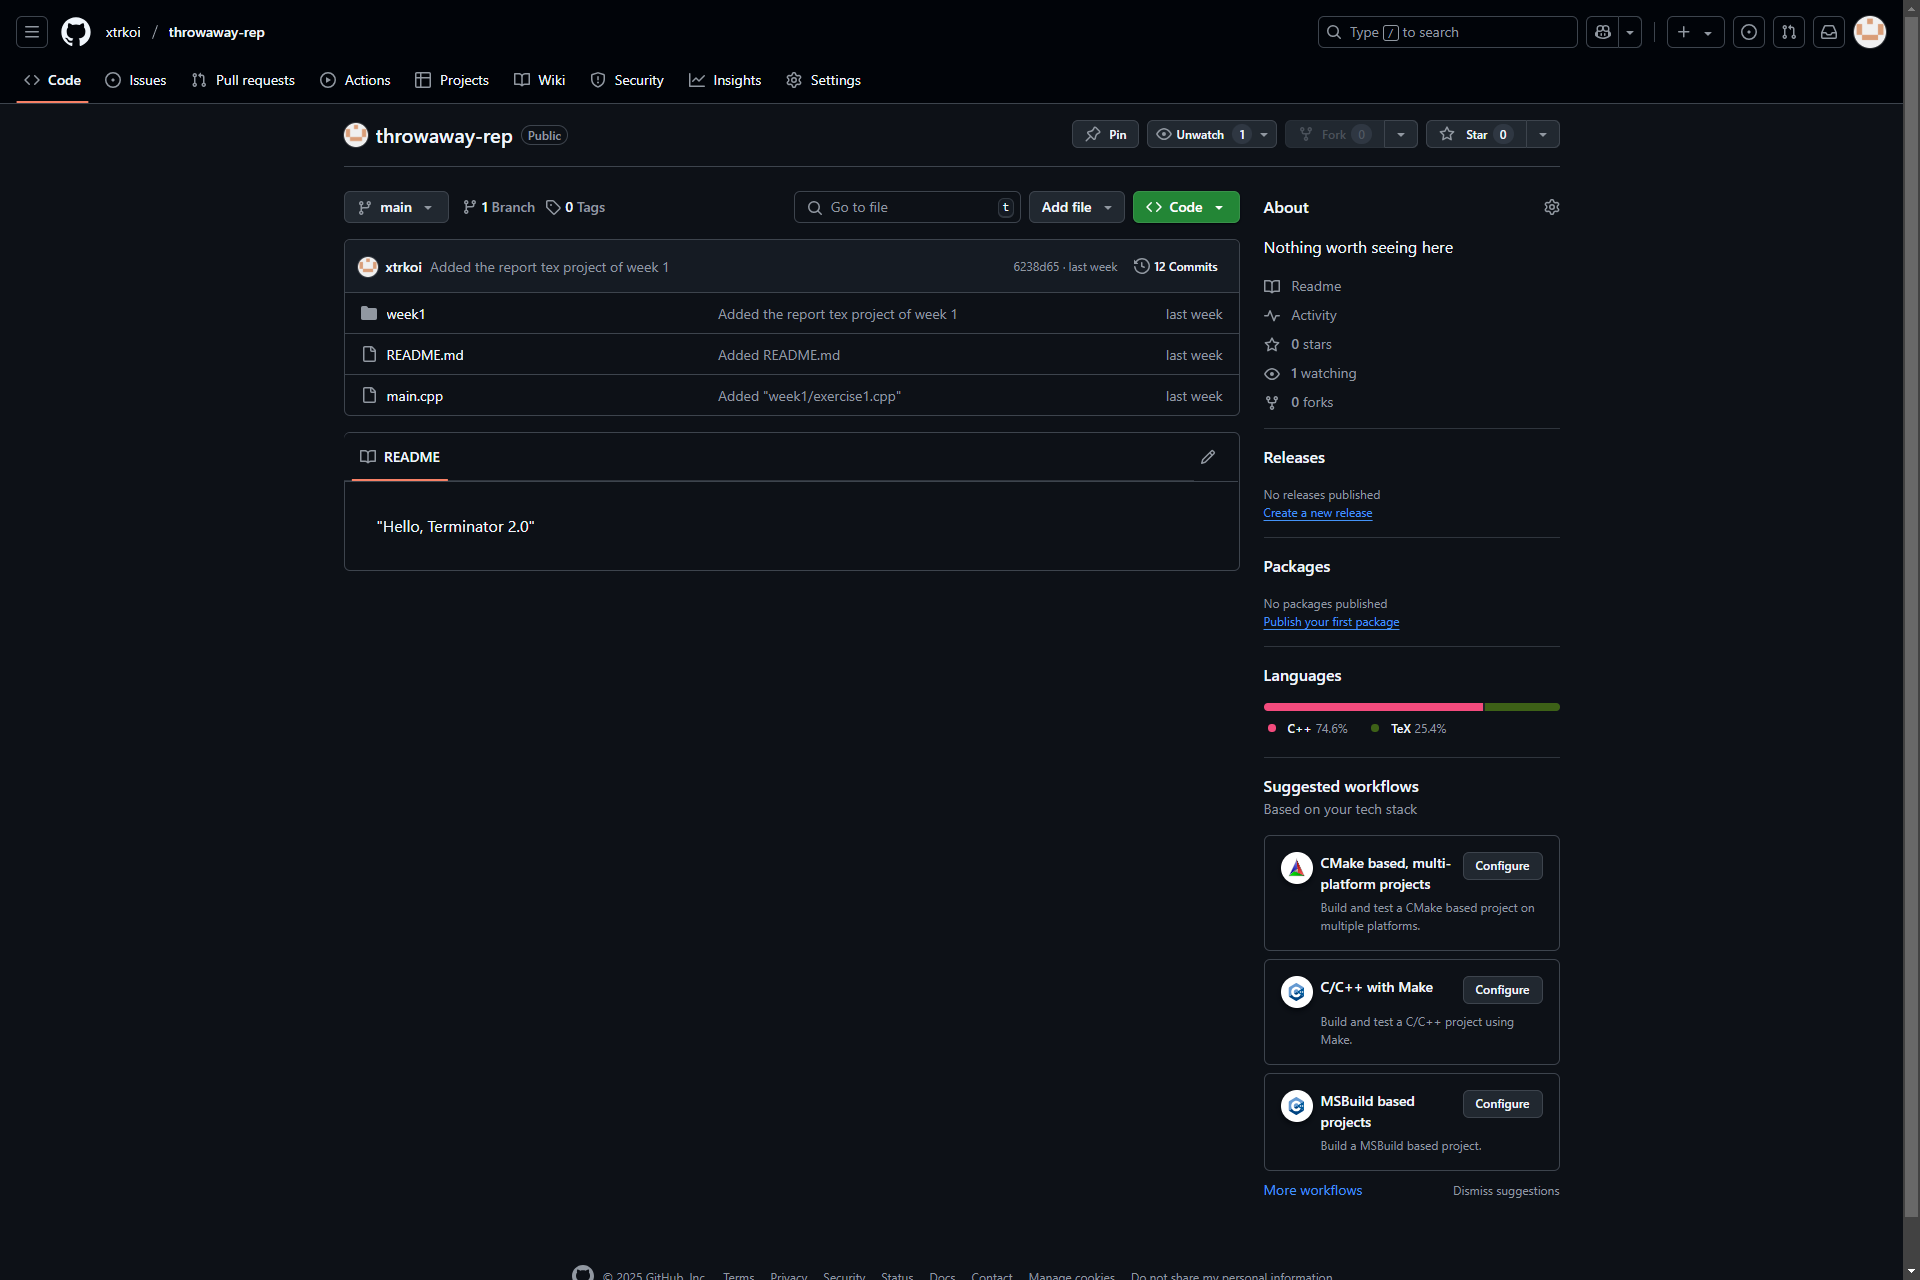
\includegraphics[width=12cm]{figure1.png}\hfil
    %     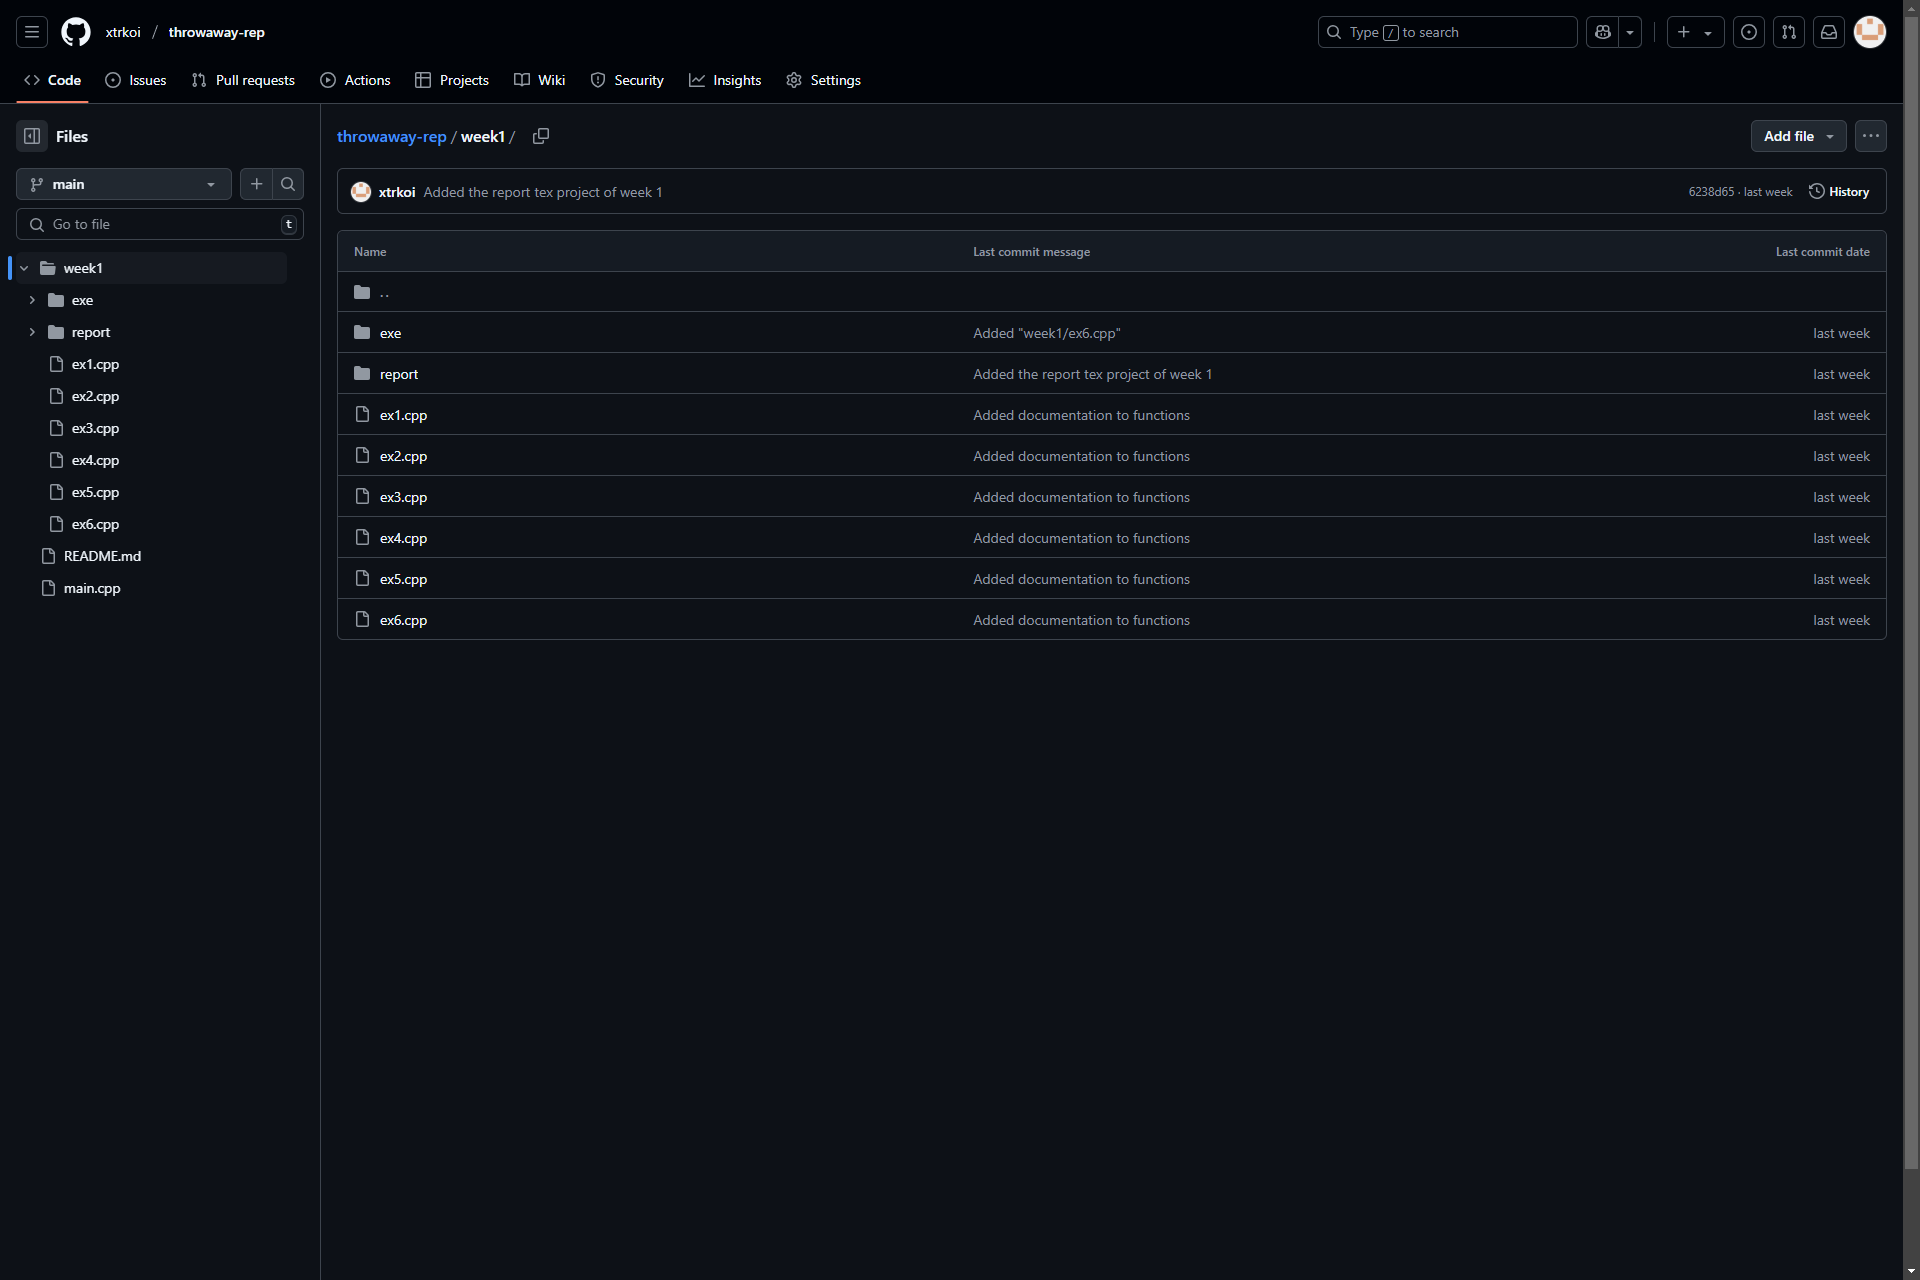
\includegraphics[width=12cm]{figure2.png}
    %     \caption{Online Github Repository}
    % \end{figure}

    \section{The Problems}



   
    \section{Conclusion}

    

\end{document}